\section{(2.g)}
In order to sort the array named 'components' in the code below, we have used the quick sort method. The pivot value in this code is chosen to be the last element. The code places  the pivot element at its correct position in sorted array and places all smaller than pivot elements to left of pivot and all greater elements to the right of it.\\

\lstinputlisting{two_g.py}

The sorted array can be found in the file \url{sortarray_2g.txt}.\\
The median, 16th and 84th percentiles for this array are as follows:

\lstinputlisting{statistics_2g.txt}

Figure \ref{fig:fig5} shows the histogram and the over plotted Poisson distribution. Although not perfect, the distributions somehow match!

\begin{figure}[!htb]
  \centering
  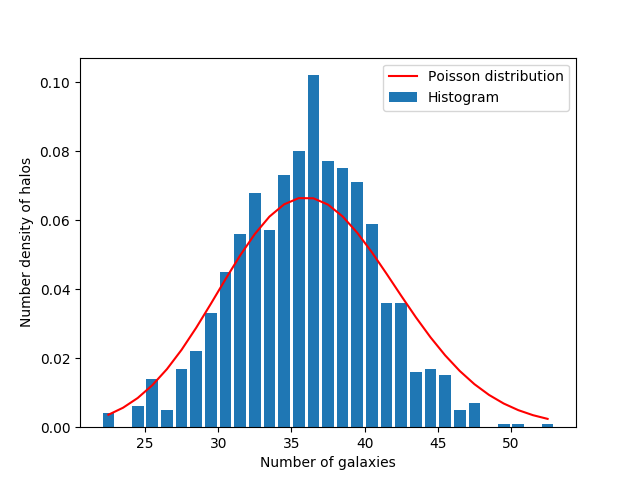
\includegraphics[width=0.7\linewidth]{Plots/distribs_2g.png}
  \caption{The galaxy number counts in 1000 halos and the relevant Poisson distribution.}
  \label{fig:fig5}
\end{figure}
